\anexo{Especificações da SELEX}
\label{an:selex_appendix}

Este documento descreve a sintaxe e a semântica da linguagem de modelagem \gls{SELEX}. A estrutura lexical e sintática é dada utilizando o \gls{EBNF}, enquanto a semântica é explicada em linguagem natural. Dado um programa, a análise lexical separa \textit{strings} (por exemplo, "\texttt{a = 2}") como tokens (por exemplo, "\texttt{a}", "\texttt{=}", "\texttt{2}"), enquanto a análise sintática opera no fluxo de \textit{tokens} e produz uma árvore sintática. Para os conceitos de alto nível na análise sintática, mais detalhes semânticos são elaborados, a fim de revelar os detalhes de semântica e implementação \cite{wonka2018}.

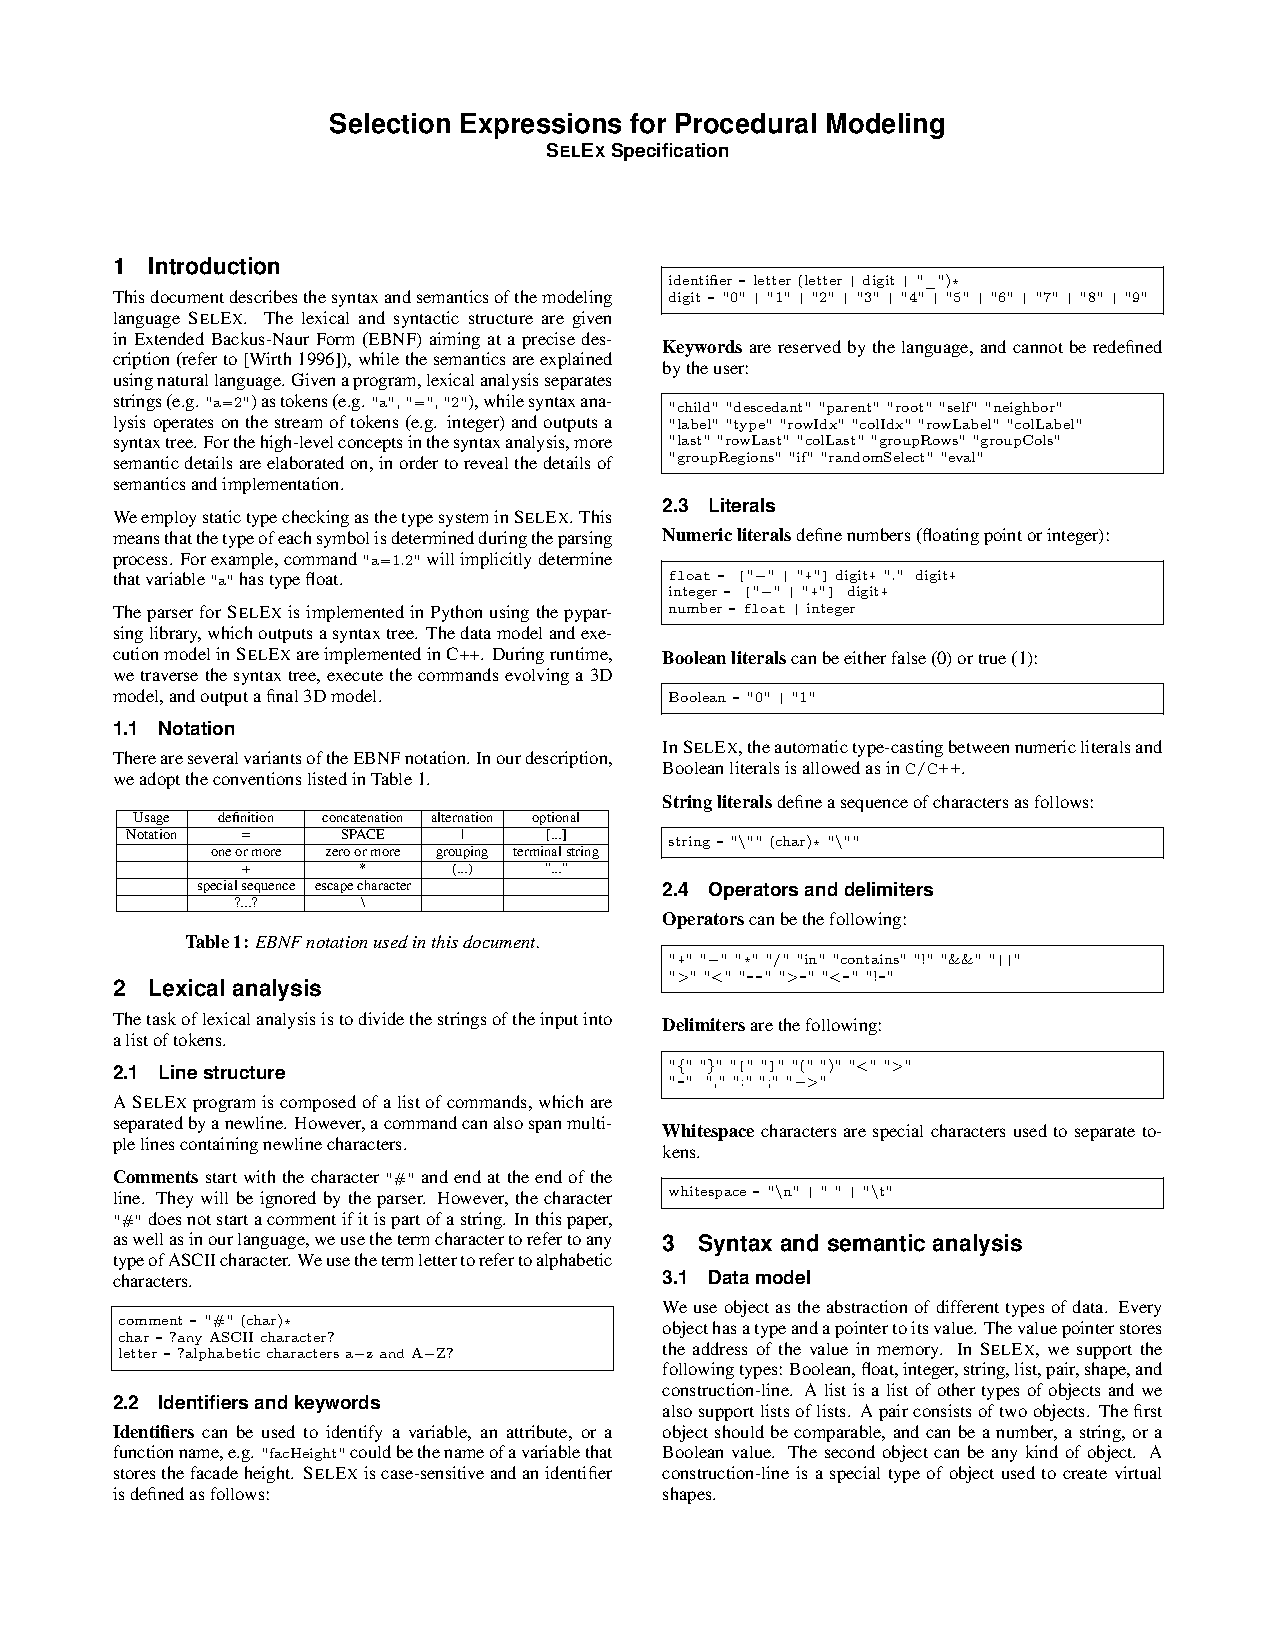
\includepdf[pages={-}]{3-pos-textuais/anexos/selex_appendix.pdf}